\subsection{Formschluss \hfill ME}
\begin{footnotesize}
    \begin{scriptsize}
        \begin{itemize}
        \item Kraftübertragung durch \textbf{Scherwiderstand}
        \item Erhöhte Kerbwirkung und Flächenpressung
        \item \textbf{Beispiele:} Stifte / Passfedern / Schrauben / Verzahnungen
        \end{itemize}
    \end{scriptsize}
    \begin{empheq}[box=\fbox]{align*}
        F \leq F_{\text{scher}} = \tau_{\text{szul}} \cdot S \quad &\mid \quad S = c \cdot A
        \\ c_{\text{eckig}} = 0.75 \quad \mid \quad c_{\text{rund}} &= 0.66 \quad \mid \quad c_{\text{hohl}} = 0.5
    \end{empheq}
    \begin{center}
        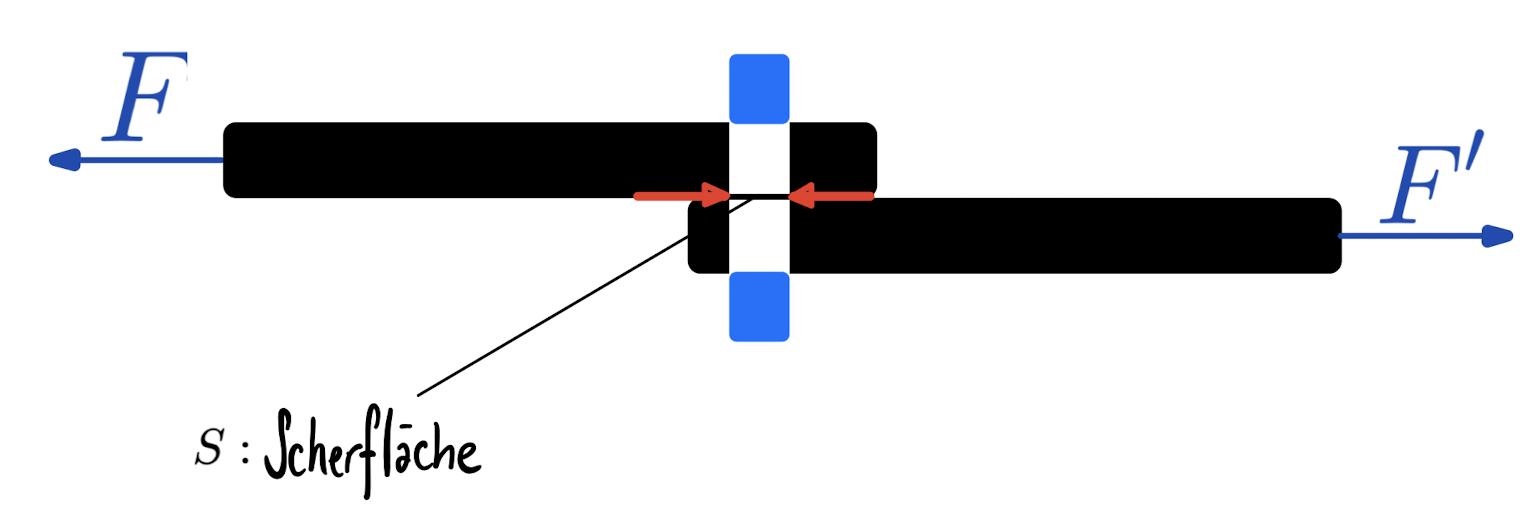
\includegraphics[width = 0.5 \linewidth]{src/images/MAEIP_Formschluss}
    \end{center}
\end{footnotesize}

\subsubsection{Passfeder \hfill ME}
\begin{scriptsize}
   \begin{itemize}
       \item \textbf{Kritische Bauteile:} Nabe, Welle $\to$ Flächenpressung, Schubspannung
   \end{itemize}
\end{scriptsize}
   \begin{minipage}{0.48\linewidth}
    \begin{center}
        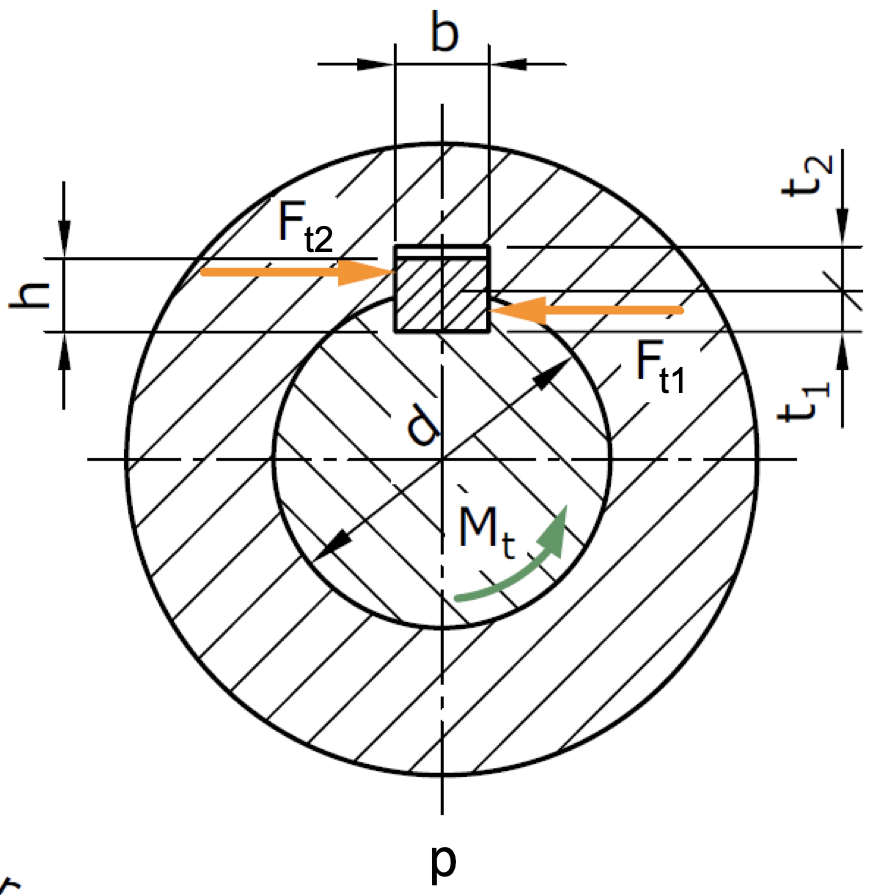
\includegraphics[width = 1.0\linewidth]{src/images/MAEIP_Passfeder}
    \end{center}
   \end{minipage}
   \begin{scriptsize}
    \begin{minipage}{0.5\linewidth}
        \begin{center}
           \begin{align*}
               p_m &= \text{Mittlere Pressung}
               \\f_s &= \text{Stützfaktor}
               \\f_h &= \text{Härteeinflussfaktor}
               \\n &= \text{Anzahl Passfedern}
               \\l_{tr}&= \text{tragende Länge}
               \\t_1 &= \text{Nuttiefe}
               \\\varphi &= \text{Traganteil} 
               \\ &= 1 \; \text{(für n=1)}
               \\ &= 0.75 \; \text{(für n=2)}
               \\c_b &= \text{Betriebsfaktor}
               \\h &= \text{Höhe}
            \end{align*}
        \end{center}
   \end{minipage}
   \end{scriptsize}
   \begin{footnotesize}
       \mathbox{
        p_{\text{zul}} = f_s \cdot f_h \cdot \frac{R_e}{S_F} = f_s \cdot \frac{R_{p0.2}}{S_F}
       }
   \end{footnotesize}
\begin{footnotesize}
\begin{empheq}[box=\fbox]{align*} 
    &M_{t, \text{max}} = \frac{p_{\text{zul}} \cdot d \cdot l_{tr}(h-t_1) \cdot n}{2} < c_b \cdot M_{\text{nenn}}
    \\ &p_m = \frac{F_U}{(h-t)\cdot l_{tr} \cdot n \cdot \varphi} = \frac{2\cdot M_t}{d\cdot(h-t) \cdot l_{tr} \cdot n \cdot \varphi} \leq p_{zul}
    \\ &\text{Form A:} \; l_{\text{tragend}} = l -(2r) = l-b
    \\ &\text{Form B:} \; l_{\text{tragend}} = l
\end{empheq}
\begin{itemize}
    \item \textbf{Wertetabelle für $c_b$:}
    \\ \hspace{-7mm}\begin{tabular}{ |c|c|c|c|c|}
        \hline
        $c_b$ & Ab &&&\\
        \hline
        An & gleichmässig & $\uparrow$ Stösse & $\uparrow \uparrow$ Stösse & $\uparrow \uparrow \uparrow$ Stösse\\
        \hline
        gleichmässig & 1.0 & 1.25 & 1.5 & 1.75\\
        \hline
        $\uparrow$ Stösse & 1.1 & 1.35 & 1.6 & 1.85\\
        \hline
        $\uparrow \uparrow$ Stösse & 1.25 & 1.5 & 1.75 & 2.0\\
        \hline
        $\uparrow \uparrow \uparrow$ Stösse & 1.5 & 1.75 & 2.0 & 2.25\\
        \hline

    \end{tabular}
    \item \textbf{Beschriftung:} DIN 6885 - $\colorbox{pink}{A} \quad \colorbox{Thistle}{14} \quad \text{x} \quad \colorbox{Apricot}{9} \quad \text{x} \quad \colorbox{Melon}{36}$
    \\ \hspace{25mm}\colorbox{pink}{Form} / \colorbox{Thistle}{Breite} / \colorbox{Apricot}{Höhe} / \colorbox{Melon}{Länge}
\end{itemize}
\end{footnotesize}

\subsubsection{Keilwelle \hfill ME}
    \begin{scriptsize}
        \begin{itemize}
            \item grose, wechselnde, stossartige Drehmomente
            \item Kerbwirkung: $\downarrow$ Biegung, $\uparrow$ Torsion $\Rightarrow$ Kosten hoch
        \end{itemize}
    \end{scriptsize}
    \begin{minipage}{0.36\linewidth}
        \begin{center}
            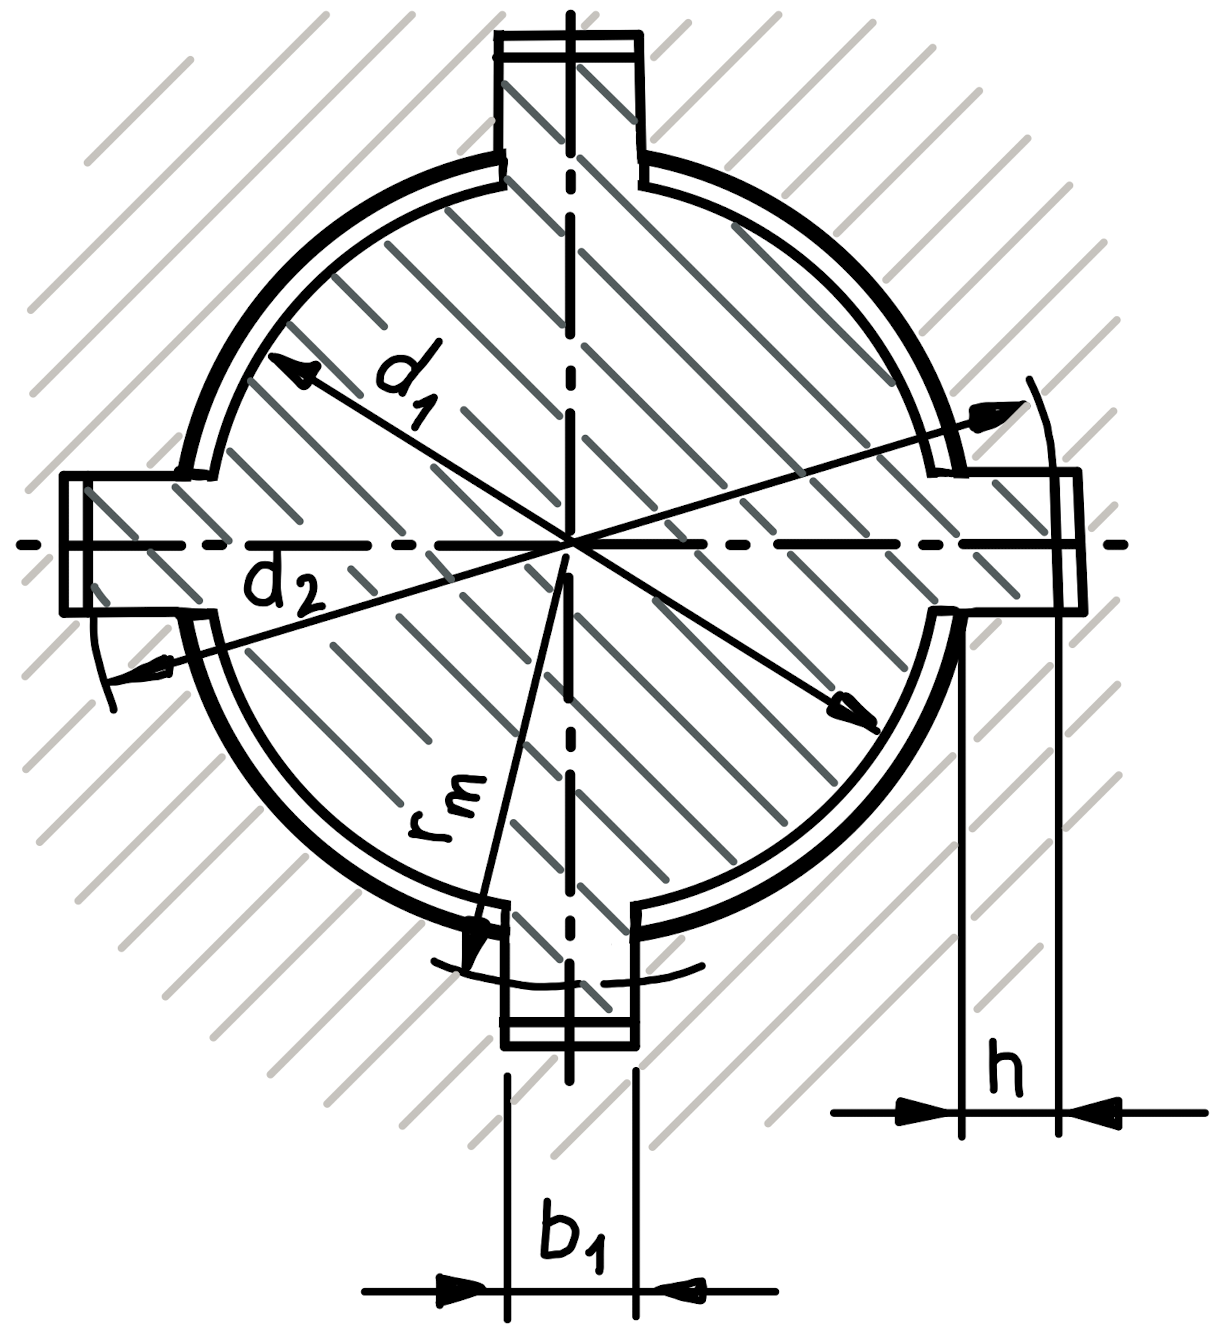
\includegraphics[width = 1.0\linewidth]{src/images/MAEIP_Keilwelle}
        \end{center}
    \end{minipage}
    \begin{minipage}{0.62\linewidth}
        \begin{center}
            \begin{scriptsize}
                \begin{align*}
                    n &= \text{Anzahl Keile}
                    \\l_{tr} = L_N &= \text{tragende Länge}
                    \\\varphi &= 0.9 \; (\text{Flankenzentrierung})
                    \\\varphi &= 0.75 \; (\text{Innenzentrierung})
                \end{align*}
            \end{scriptsize}
            \begin{footnotesize}
                \begin{empheq}[box=\fbox]{align*}
                    r_m &= \frac{d_1 + d_2}{4}
                    \\h &= 0.5 \cdot (d_{2,W} -d_{1,N})
                    \\h_{tr} &\approx 0.4 \cdot (d_{2} - d_{1})
                    \\M_{t, \text{max}} &= h_{tr} \cdot l_{tr} \cdot p_{\text{zul}} \cdot r_m \cdot \varphi \cdot n
                    \\p_m &= \frac{10 \cdot M}{(D+d) l_{tr} (D-d) n \cdot \phi}
                \end{empheq}
            \end{footnotesize}
        \end{center}
    \end{minipage}